\section{S6 -- Architektura warstwowa w internetowych aplikacji bazodanowych}

Jeżeli mówimy o architekturze warstwowej (ang. \textit{tier architectrue}) to zawsze mamy na myśli architekturę n warstwową, gdzie n > 0. Najbardziej popularne architektury warstwowe to:

\begin{itemize}
	\setlength\itemsep{1pt}
	\item \textbf{Architektura jednowarstwowa} - całe oprogramowanie zamknięte jest w jednej "warstwie". Przykładem są proste aplikacje desktopowe.
	\item \textbf{Architektura dwuwarstwowa} - oprogramowanie podzielone jest na dwie warstwy - przykładem architektury dwuwarstwowej jest klient-serwer. Oprogramowanie klienta to jedna warstwa a serwera druga. 
	
	\begin{figure}[H]
		\centering
		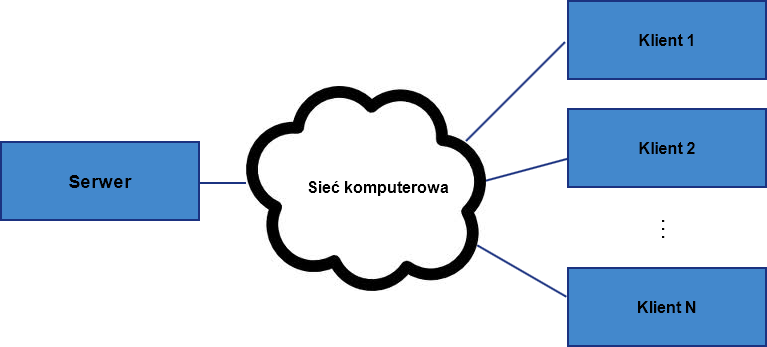
\includegraphics[scale=0.5]{s2_klient_serwer.png}
		\caption{Architektura klient-serwer}
	\end{figure}
	
	Komunikacja pomiędzy serwerem oraz klientami odbywa się za pomocą konkretnego protokołu rozumianego zarówno przez serwer jak i klienta. Mogą to być standardowe protokoły typu np. HTTP, SMTP, FTP.... lub dedykowane - zaprojektowane na potrzeby konkretnego rozwiązania.
	
	Klient z reguły zawiera interfejsy użytkownika, a serwer posiada dostęp do bazy danych. Serwer to nie tylko skomplikowana dedykowana aplikacja na potrzeby jakiegoś rozwiązania. Rolę serwera może pełnić np. RDBMS bez dodatkowej logiki aplikacyjnej.
	
	Najbardziej popularne dzisiaj rozwiązania architektury klient-serwer to oczywiście sieć www, gdzie rolę serwerów pełnią serwery www a rolę klientów: przeglądarki internetowe.
	\item \textbf{Architektura trójwarstwowa} - w architekturze tej wyróżnia się następujące warstwy:
	
	\begin{itemize}
		\setlength\itemsep{1pt}
		\item \textbf{Warstwa prezentacji} (ang. \textit{presentation tier}) - odpowiedzialna za interakcję z użytkownikiem końcowym (wyświetlanie i wprowadzanie danych). W tej warstwie działają aplikacje klienckie takie jak np. przeglądarki internetowe 
		\item \textbf{Warstwa biznesowa} (ang. \textit{business tier}) - odpowiedzialna za przetwarzanie danych (żądań) od użytkownika.  Tutaj też przygotowywane są dane wysłane  do warstwy prezentacji (aplikacji klienckich). W tej warstwie realizowane są wszelkiego rodzaju funkcjonalności biznesowe. Z drugiej strony logika warstwy odpowiedzialna jest za komunikację z warstwą danych. Warstwa biznesowa stanowi swego rodzaju pomost pomiędzy warstwą aplikacji i warstwą danych dodając elementy przetwarzania.
		\item \textbf{Warstwa danych} (ang. \textit{persistance tier}) - odpowiedzialna za przechowywane danych. W tej warstwie mamy np. bazę danych.
	\end{itemize}

	\begin{figure}[H]
		\centering
		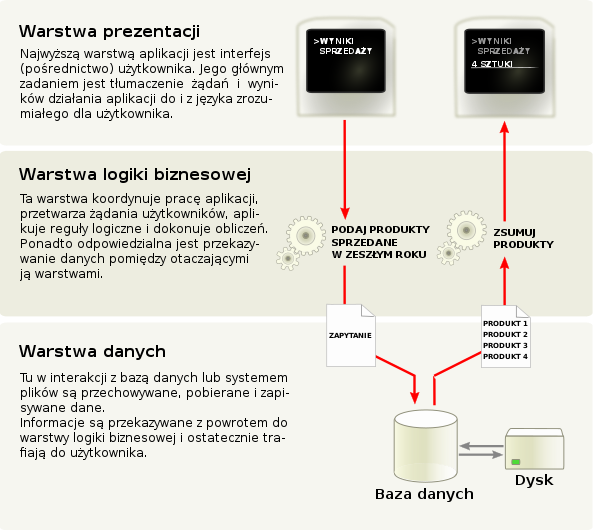
\includegraphics[scale=0.65]{s2_3warstwy.png}
		\caption{Architektura trójwarstwowa}
	\end{figure}

\end{itemize}

\begin{itemize}
	\setlength\itemsep{1pt}
	\item[] \textbf{Zalety podziału architektury na warstwy:}
	\item podział na niezależne komponenty, 
	\item łatwość podmiany, 
	\item rozdzielenie całego systemu na dedykowane dla danej warstwy zadania, 
	\item ułatwia skalowanie i zarządzanie.
\end{itemize}